%#########################################

% author: S. Parisa Daj.
% email: s.dajkhosh@memphis.edu
% University of Memphis
% Sep 2021

%#########################################

\documentclass[12pt,oneside,geqno]{article}

\addtolength{\textheight}{120pt}
\oddsidemargin=-10pt
\topmargin=-.5in
\textwidth=6.5in
\pagestyle{empty}

% ######################## 	Packages
\usepackage{amssymb,latexsym,amsmath,amsthm}
\usepackage{amsfonts,raWFonts}
\usepackage{thmtools}
\usepackage{systeme}
\usepackage{mathtools}
\usepackage[usenames,dvipsnames]{color}
\usepackage{xcolor}
\usepackage{xfrac}
\usepackage{hyperref}
\usepackage[utf8]{inputenc}
\usepackage{enumerate}



\usepackage{listings}
\usepackage{xcolor}

\usepackage{graphicx}
\usepackage{caption}
\usepackage{subcaption}

% ######################## 	Colors
\definecolor{codegreen}{rgb}{0,0.6,0}
\definecolor{codegray}{rgb}{0.5,0.5,0.5}
\definecolor{codepurple}{rgb}{0.58,0,0.82}
\definecolor{backcolour}{rgb}{0.97,0.97,0.95}

% ######################## 	Style
\lstdefinestyle{mystyle}{
	backgroundcolor=\color{backcolour},   
	commentstyle=\color{codegreen},
	keywordstyle=\color{magenta},
	numberstyle=\tiny\color{codegray},
	stringstyle=\color{codepurple},
	basicstyle=\ttfamily\footnotesize,
	breakatwhitespace=false,         
	breaklines=true,                 
	captionpos=b,                    
	keepspaces=true,                 
	numbers=left,                    
	numbersep=5pt,                  
	showspaces=false,                
	showstringspaces=false,
	showtabs=false,                  
	tabsize=2
}

\lstset{style=mystyle}

\declaretheoremstyle[
headfont=\color{blue}\normalfont\bfseries,
notefont=\bfseries, 
notebraces={}{},
%bodyfont=\color{red}\normalfont\itshape,
bodyfont=\normalfont,%\itshape,
%headformat=\NUMBER.~\NAME\NOTE
headformat=\NAME\NOTE
]{colorejercicio}

\declaretheorem[
%numbered=no,
style=colorejercicio,
name=Problem
]{Problem}

% ######################## 	Document
\begin{document}
	
	\begin{center}
		{\LARGE EECE 8740-Neural Networks HW \#2}% Title
		\vspace*{1\baselineskip}   
		
		\scshape % Small caps
		\color{red}{(Solutions)}\\
		%  
		\vspace*{1\baselineskip}
		\color{black}University of Memphis\\[\baselineskip]
		%
		\vspace*{5\baselineskip} 
		
		Written by \\[\baselineskip]
		{\Large S. Parisa Daj.\par U00743495} \\
		(s.dajkhosh@memphis.edu)\\
		
		\vspace*{1\baselineskip}
		\today
	\end{center}
	%
	\clearpage
	
	%%%%%%%%%%%%%%%%%%%					1_question
	\begin{Problem}[a]
		Question
		Design a convolutional neural network (CNN) model considering the following criteria:
		
		\begin{enumerate}[a) ]
			\item Design a CNN model with (fig \ref{img:q1_net}) configuration.
			\begin{figure}
				\centering
				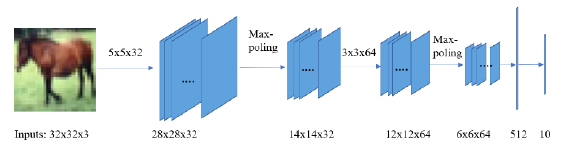
\includegraphics[width=\textwidth]{../figs/q1_net.png}
				\caption{Network architecture for the first question.}
				\label{img:q1_net}
			\end{figure}
			
			\item Activation functions: ReLU
			\item Batch normalization
			\item Use SoftMax layer for classification
			\item Number of epochs: 100 and
			\item Batch-size is 32 (you can increase or decrease the batch size if required).
			\item Optimizer: SGD with a learning rate and momentum.
		\end{enumerate}
		
		Evaluate the model on CIFAR-10 dataset:
		
		\begin{enumerate}[a) ]			
			\item Input image: 32x32x3 pixels (RGB images)
			\item Number of training samples: 50,000
			\item Number of testing samples: 10,00
			\item Number of classes: 10 (different objects).
		\end{enumerate}
		
		Write a report including training logs, testing errors or accuracy, computational times, etc.
		
	\end{Problem}
	
	%%%%%%%%%%%%%%%%%%%					1_solution
	\begin{proof}[\color{red}{Solution}]
		
		\section{Introduction}
		
		Regarding the question, the first step is to download the CIFAR-20 dataset directly from Keras, which has 60000 samples. 50000 samples are used to train the model, and the rest are for the evaluation. The goal of this problem is to classify these pictures of objects labeled in 10 different classes. Input images are \(32*32\), and as they are in RGB mode, there will be three channels, meaning that the input size will be \(32*32*3\). Also considering the number of classes, the output layer will contain ten neurons.
		\begin{figure}
			\centering
			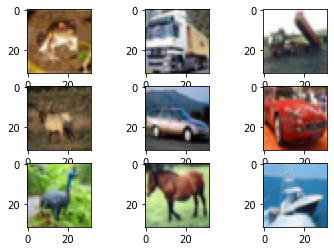
\includegraphics[width=\textwidth]{../figs/q1_sample.png}
			\caption{Sample first 9 images from the CIFAR dataset.}
			\label{img:q1_sample}
		\end{figure}
		
		\section{Methodology and Deep Learning Architecture}
		The architecture of this network as given in (fig \ref{img:q1_net}) includes a combination of convolutional neural networks and pooling layers using the ReLU activation function. The final convolutional layer would be the feature layer. By passing it through a flattened layer followed by a fully connected layer, the features are formed in one dimension. And the final layer includes neurons equal to the number of classes. Then, the outputs are normalized by passing a SoftMax activation function. 
		To go into more details, applying a \(5*5*32\) convolutional filter to the \(32*32*3\) input, without any padding and strides, considering that \(output size = \frac{input size + 2 * padding - number of channels}{strides} + 1\) will give an output with the size of \(26*26*32\) from the first convolutional layer. Following the layers, to have an output size of \(14*14*32\) for the second layer, the max-pooling layer will have a pooling size of \((2, 2)\)). In the same way, the third layer includes a \(3*3*64\) convolutional layer to give an output of \(12*12*64\), followed by a \((2, 2)\) max-pooling layer. By going deeper, the goal is to find the features more accurately. Then, to reach out the outputs, the output of the final convolutional layer will pass across a flattened layer to be in one dimension, followed by a fully connected layer of 512 neurons, finally, the output fully connected layer with ten neurons will be applied using the SoftMax activation functions which its goal is to limit the output values as probabilities between 0 and 1. 
		As mentioned in the question, Stochastic Gradient Descent Optimizer is being used in this network as an experiment. However, I believe that Adam Optimizer will result in a more accurate evaluation. The process has a batch size of 32 and is training in 100 iterations. All this is done using GPU-based Google Colaboratory in almost 1000 seconds (10 seconds per iteration). The batch normalization layers are added before each max-pooling layer to avoid over-fitting. 
		
		\section{Experimental and Test Results}
		
		Two experiments have been completed to evaluate the final model. Firstly, the network does not include batch normalization layers shown in (fig \ref{img:q1_log})) maximum accuracy maintained in this experiment is 69.1 percent on the validation set. In the next trial, two batch normalization layers are added, before each max-pooling layer. Adding these two layers, as expected resulted in higher accuracy (71.9 percent) as presented in (fig \ref{img:q1_log_batch}). Regarding the two figures, it is concluded that both of these networks are reaching a specific accuracy, and keep staying in the same amount after around 20 epochs, although the loss function starts to increase after that epoch. However, the training accuracy is increasing to 100 percent. Meaning that the process is memorizing the training set instead of learning it, which results in over-fitting. 
		\begin{figure}
			\centering
			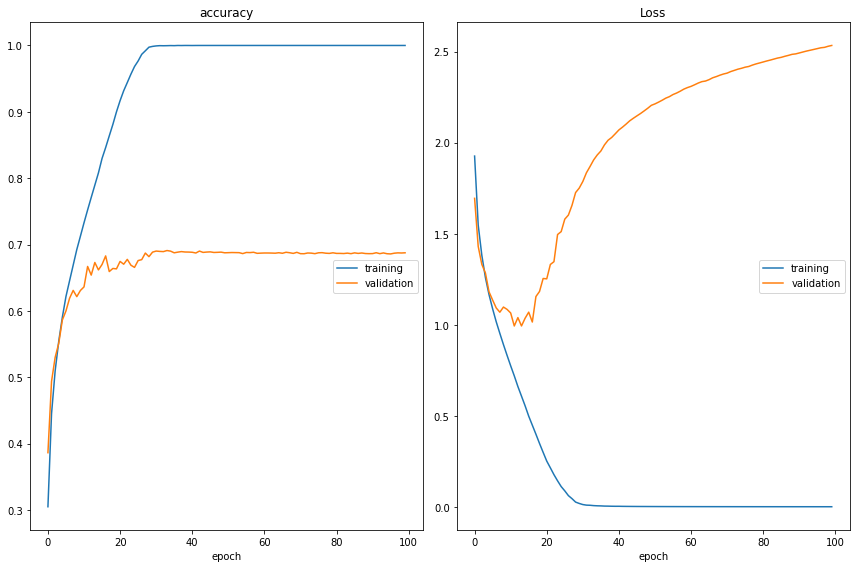
\includegraphics[width=\textwidth]{../figs/q1_acc, loss.png}
			\caption{Network train and validation accuracy and loss logs along the epochs.}
			\label{img:q1_log}
		\end{figure}
		
		\begin{figure}
			\centering
			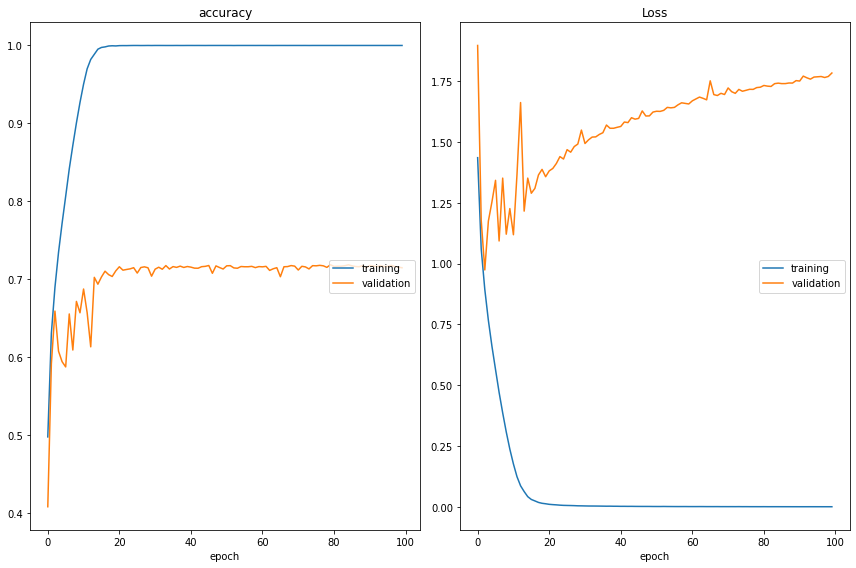
\includegraphics[width=\textwidth]{../figs/q1_acc, loss_batchnormalization.png}
			\caption{Network train and validation accuracy and loss logs along the epochs.}
			\label{img:q1_log_batch}
		\end{figure}
		\section{Conclusion}
		After applying the network on the dataset, it looks like that after a specific value for accuracy, over-fitting is happening, and the further iterations seem to be useless. To avoid this issue, maybe more batch normalization layers are needed to be combined with some dropout layers to increase the stochastic behavior of the data. Also, the over-fitting shows that the curve fitted to the data points is set very accurately on the data points of the training set. Meaning that the complexity of the system might be high for these data points. Therefore, one possible solution would be to decrease the complexity of the network by having a network less deep or with fewer neurons.
		\href{https://colab.research.google.com/drive/1vs7KYJjMphoGcK-9g3tKnQ49ZFdIiYI5#scrollTo=ydX8Mu84z5oD}{Link for the code to this solution}
	\end{proof}
	
	%%%%%%%%%%%%%%%%%%%					2_question
	\begin{Problem}[b]
		This assignment aims to develop a Deep Convolutional Neural Networks (DCNN) model and achieve better accuracy for scene understanding or classification tasks.
		
		Download the datasets and prepare as required for training and testing. You can resize the data to 32x32 or 64x64 (depending on the availability of hardware). Use 70% of samples for training and the remaining 30% for testing per category.
		
		\begin{itemize}
			
			\item Implement a DCNN model, which provides better recognition accuracy for the scene classification tasks. For designing a DCNN model, consider the following criteria:
			
			\begin{enumerate}[a)]
				
				\item Data augmentation
				\item Better initialization methods(for example:Xavier and He initializer)
				\item Activation function:ELU
				\item Dropout (Regularization)
				\item Batch normalization
				
			\end{enumerate}
			
			
			
			\item Evaluated the performance of the model for different optimization function:
			\begin{enumerate}[a)]
				\item SGD
				\item Adam
				\item RMSProp
				
			\end{enumerate}
			
			\item Write a report including training logs (accuracy and losses), testing accuracy, computational times, and comparison for different optimization and initialization methods. 
		\end{itemize}
		
		\begin{figure}
			\centering
			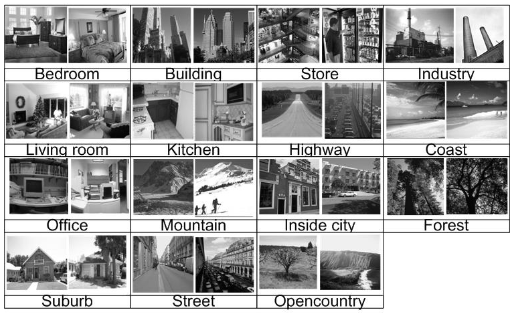
\includegraphics[width=\textwidth]{../figs/q2_classes.png}
			\caption{Sample images from all classes in 15-Scene dataset.}
			\label{img:q2_classes}
		\end{figure}
	\end{Problem}
	
	%%%%%%%%%%%%%%%%%%%					2_solution
	\begin{proof}[\color{red}{Solution}]
		
		\section{Introduction}
		\renewcommand*{\theHsection}{chX.\the\value{section}}
		The goal of this assignment is to design a deep convolutional neural network. To do so, some information has been gathered from lectures 7 to 9 and the codes provided for them by Professor Zahangir. The network will be trained on the 15-Scene dataset available at Kaggle. There are 4485 images available in this dataset that represent 15 various scenes.
		
		\begin{figure}
			\centering
			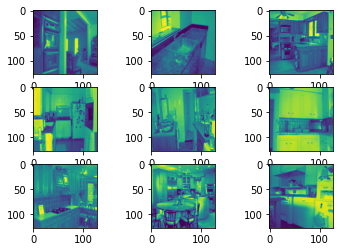
\includegraphics[width=\textwidth]{../figs/q2_sample.png}
			\caption{Sample first 9 images from the 15-Scene dataset.}
			\label{img:q2_sample}
		\end{figure}
		
		
		\section{Methodology and Deep Learning Architecture}
		First of all, training and testing datasets have to be split. The dataset is downloaded in 15 different folders regarding 15 classes. Each image is black and white and two-dimensional. The input size varies image by image between 203 to 304 pixels per side. As a result, they have to be resized to similar sizes. As suggested in the question, sizes 128, 64, or 32 are recommended. Because of the computation saving, the input sizes of 32 and 64 pixels have been tested. However, finally, the best results were achieved by images of \(128*128\) pixels. In the next step, to split the training and validations sets, each folder is treated individually to have equal percentages of each class. Thirty percent of each class is separated as the validation set. As a result, 3133 pictures are used to train the model. Then, the model is validated on 1352 images that have not seen the model before. 
		The network architecture is shown in (table \ref{tab:arch}).  
		
		\begin{table}[]
			\caption{The introduced architecture for this design.}
			\label{tab:arch}
			\begin{tabular}{lll}
				\hline
				\multicolumn{1}{|l|}{Layer (type)}                  & \multicolumn{1}{l|}{Output Shape} & \multicolumn{1}{l|}{Param \#} \\ \hline
				conv2d (Conv2D)                                     & (None, 128, 128, 32)              & 320                           \\
				activation (Activation)                             & (None, 128, 128, 32)              & 0                             \\
				batch\_normalization (BatchNo (None, 128, 128, 32)  & 128                               &                               \\
				conv2d\_1 (Conv2D)                                  & (None, 128, 128, 32)              & 9248                          \\
				activation\_1 (Activation)                          & (None, 128, 128, 32)              & 0                             \\
				batch\_normalization\_1 (Batch (None, 128, 128, 32) & 128                               &                               \\
				max\_pooling2d (MaxPooling2D) (None, 64, 64, 32)    & 0                                 &                               \\
				dropout (Dropout)                                   & (None, 64, 64, 32)                & 0                             \\
				conv2d\_2 (Conv2D)                                  & (None, 64, 64, 64)                & 18496                         \\
				activation\_2 (Activation)                          & (None, 64, 64, 64)                & 0                             \\
				batch\_normalization\_2 (Batch (None, 64, 64, 64)   & 256                               &                               \\
				conv2d\_3 (Conv2D)                                  & (None, 64, 64, 64)                & 36928                         \\
				activation\_3 (Activation)                          & (None, 64, 64, 64)                & 0                             \\
				batch\_normalization\_3 (Batch (None, 64, 64, 64)   & 256                               &                               \\
				max\_pooling2d\_1 (MaxPooling2 (None, 32, 32, 64)   & 0                                 &                               \\
				dropout\_1 (Dropout)                                & (None, 32, 32, 64)                & 0                             \\
				conv2d\_4 (Conv2D)                                  & (None, 32, 32, 128)               & 73856                         \\
				activation\_4 (Activation)                          & (None, 32, 32, 128)               & 0                             \\
				batch\_normalization\_4 (Batch (None, 32, 32, 128)  & 512                               &                               \\
				conv2d\_5 (Conv2D)                                  & (None, 32, 32, 128)               & 147584                        \\
				activation\_5 (Activation)                          & (None, 32, 32, 128)               & 0                             \\
				batch\_normalization\_5 (Batch (None, 32, 32, 128)  & 512                               &                               \\
				max\_pooling2d\_2 (MaxPooling2 (None, 16, 16, 128)  & 0                                 &                               \\
				dropout\_2 (Dropout)                                & (None, 16, 16, 128)               & 0                             \\
				conv2d\_6 (Conv2D)                                  & (None, 16, 16, 256)               & 295168                        \\
				activation\_6 (Activation)                          & (None, 16, 16, 256)               & 0                             \\
				batch\_normalization\_6 (Batch (None, 16, 16, 256)  & 1024                              &                               \\
				conv2d\_7 (Conv2D)                                  & (None, 16, 16, 256)               & 590080                        \\
				activation\_7 (Activation)                          & (None, 16, 16, 256)               & 0                             \\
				batch\_normalization\_7 (Batch (None, 16, 16, 256)  & 1024                              &                               \\
				max\_pooling2d\_3 (MaxPooling2 (None, 8, 8, 256)    & 0                                 &                               \\
				dropout\_3 (Dropout)                                & (None, 8, 8, 256)                 & 0                             \\
				conv2d\_8 (Conv2D)                                  & (None, 8, 8, 512)                 & 1180160                       \\
				activation\_8 (Activation)                          & (None, 8, 8, 512)                 & 0                             \\
				batch\_normalization\_8 (Batch (None, 8, 8, 512)    & 2048                              &                               \\
				conv2d\_9 (Conv2D)                                  & (None, 8, 8, 512)                 & 2359808                       \\
				activation\_9 (Activation)                          & (None, 8, 8, 512)                 & 0                             \\
				batch\_normalization\_9 (Batch (None, 8, 8, 512)    & 2048                              &                               \\
				max\_pooling2d\_4 (MaxPooling2 (None, 4, 4, 512)    & 0                                 &                               \\
				dropout\_4 (Dropout)                                & (None, 4, 4, 512)                 & 0                             \\
				flatten (Flatten)                                   & (None, 8192)                      & 0                             \\
				dense (Dense)                                       & (None, 15)                        & 122895                        \\
				activation\_10 (Activation)                         & (None, 15)                        & 0                            
			\end{tabular}
		\end{table}
		
		In this architecture, there are 4,842,479 total number of parameters that 4,838,511 of them are trainable parameters.
		
		
		\section{Experimental and Test Results}
		
		This network is applied with three different optimizers (SGD, RMSProp, and Adam) in 50 epochs. The activation function for all layers except the output layer is Elu. Also, the output layer includes 15 layers equal to the 15 scene classes with a SoftMax activation function. Batch normalization and dropout layers are added to increase efficacy. For weight initialization also, the "He" initializer is utilized. After a few trials and changes in the learning rate for all experiments they are chosen to be 0.01 initially, and decay until \(10^-6\).
		
		The stochastic gradient descent optimizer without data augmentation results in a maximum of 59.3 percent validation accuracy (fig \ref{img:sgd}). After applying data augmentation, the maximum accuracy is 49.3, which is unexpected (fig \ref{img:sgd_aug}). The progress shows that maybe in later epochs, a higher validation accuracy will be achieved.
		
		\begin{figure}
			\centering
			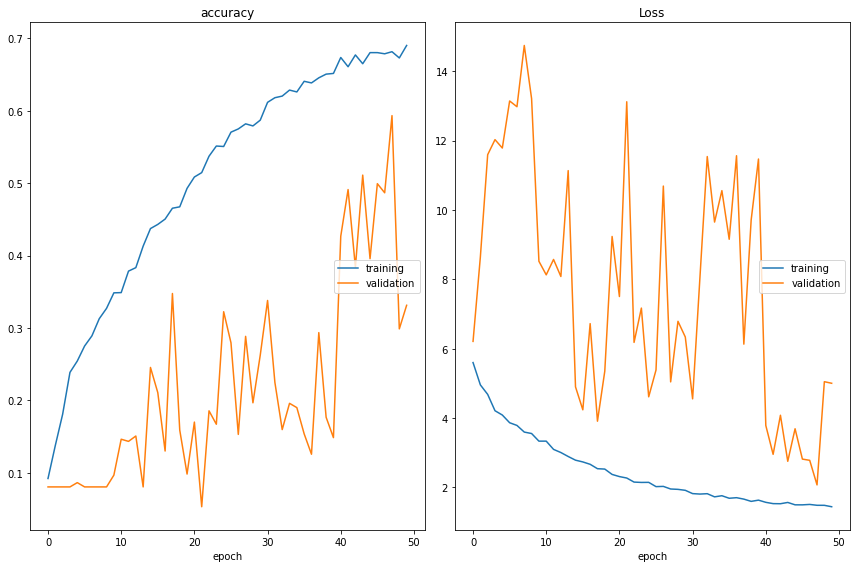
\includegraphics[width=\textwidth]{../figs/sgd_acc_loss.png}
			\caption{Accuracy and Loss of the model using Stochastic Gradient Descent Optimization Algorithm without Augmentation.}
			\label{img:sgd}
		\end{figure}
		
		\begin{figure}
			\centering
			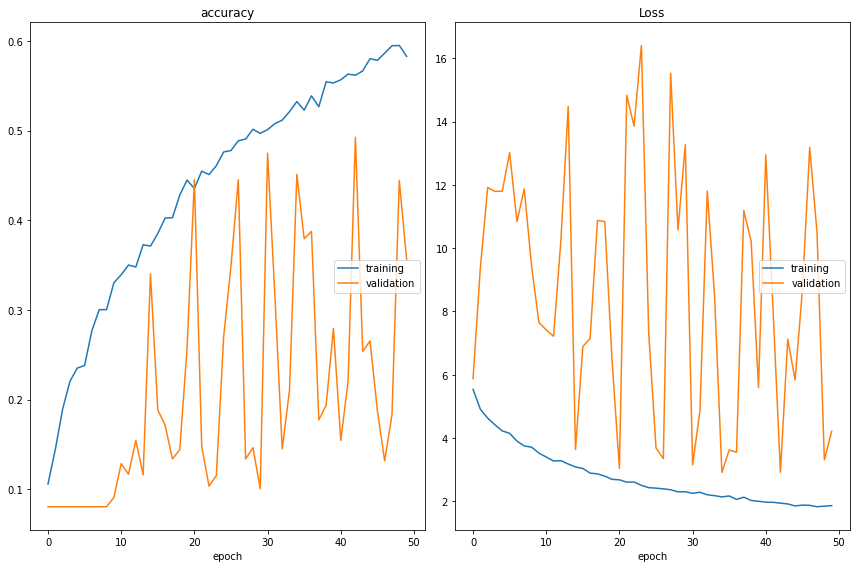
\includegraphics[width=\textwidth]{../figs/sgd_aug_acc_loss.png}
			\caption{Accuracy and Loss of the model using Stochastic Gradient Descent Optimization Algorithm using Augmentation.}
			\label{img:sgd_aug}
		\end{figure}
		
		The next optimizer is RMS-Prop which results in maximum 27.7 percent validation accuracy (fig \ref{img:rmsprop}. By using data augmentation, 35.1 will be the highest percentage for the accuracy (fig \ref{img:rmsprop_aug}). The increase in the accuracy makes sense since the number of training and testing data is increased. Therefore, the training would perform more efficiently. The figures for this optimizer show that the fluctuations of accuracy and loss change are more moderate using the RMS-Prop optimizer. However, they are not as efficient as the two other optimizers.
		
		\begin{figure}
			\centering
			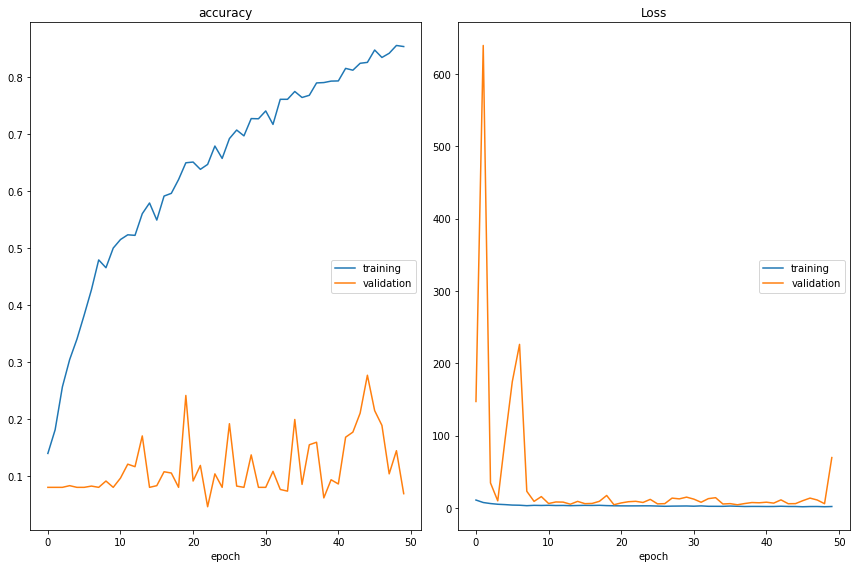
\includegraphics[width=\textwidth]{../figs/rmsprop_acc_loss.png}
			\caption{Accuracy and Loss of the model using RMSProp Optimization Algorithm without Augmentation.}
			\label{img:rmsprop}
		\end{figure}
		
		\begin{figure}
			\centering
			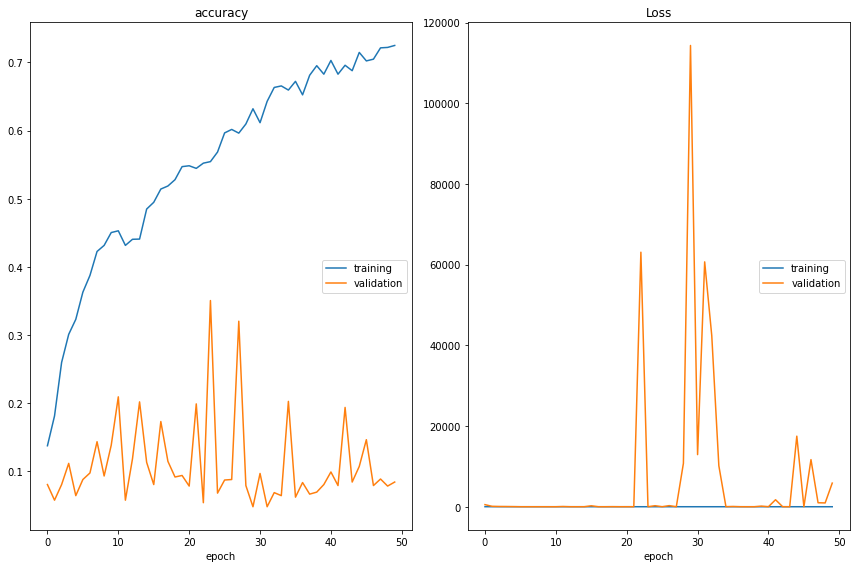
\includegraphics[width=\textwidth]{../figs/rmsprop_aug_acc_loss.png}
			\caption{Accuracy and Loss of the model using RMSProp Optimization Algorithm using Augmentation.}
			\label{img:rmsprop_aug}
		\end{figure}
		
		Finally, the maximum accuracy gained with Adam optimizer for the pure dataset and the augmented dataset are 62.4 and 63.7 percent shown in (fig \ref{adam}) and (fig \ref{img:adam_aug}). Furthermore, as these two networks reached the highest accuracy among the previous two optimizers, I decided to train the model in 100 iterations for this optimizer once again. As expected the accuracy has increased to 70.4 percent (fig \ref{img:adam_100}) for the training without data augmentation, and 72.8 percent (fig \ref{img:adam_aug_100}) when augmenting the data. 
		%		128:  
		%			sgd: max: 59.3: 10 min
		%		surprisingly: maybe I needed to clear everything! I do not know: cross validation
		
		\begin{figure}
			\centering
			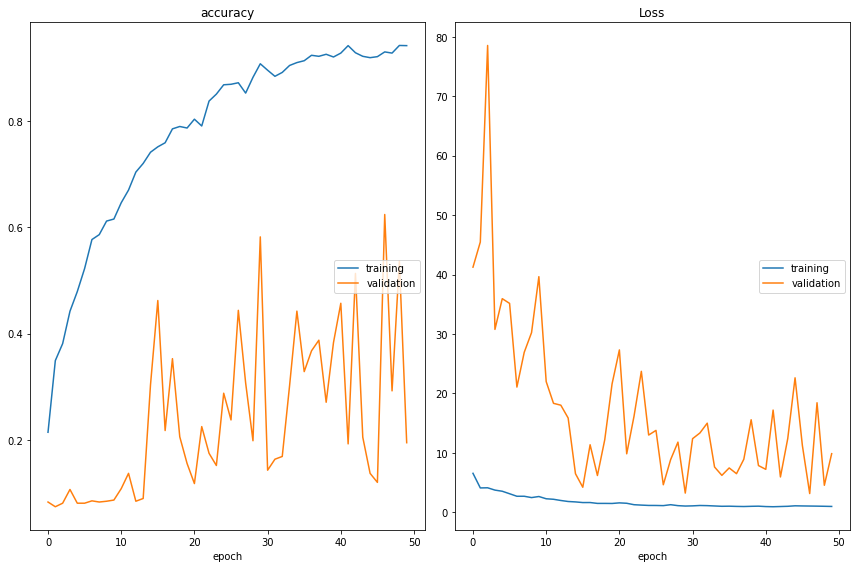
\includegraphics[width=\textwidth]{../figs/adam_acc_loss.png}
			\caption{Accuracy and Loss of the model using Adam Optimization Algorithm without Augmentation.}
			\label{img:adam}
		\end{figure}
		
		\begin{figure}
			\centering
			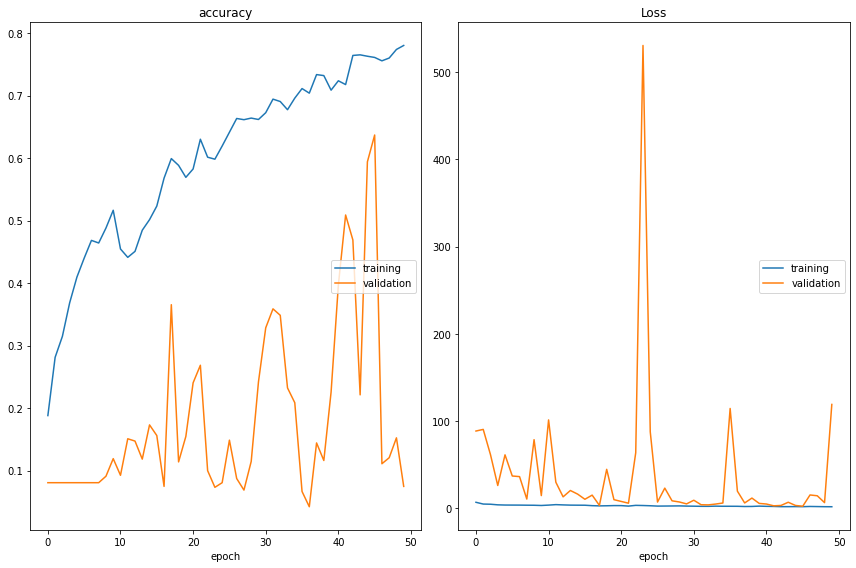
\includegraphics[width=\textwidth]{../figs/adam_aug_acc_loss.png}
			\caption{Accuracy and Loss of the model using Adam Optimization Algorithm using Augmentation.}
			\label{img:adam_aug}
		\end{figure}
		
		
		\begin{figure}
			\centering
			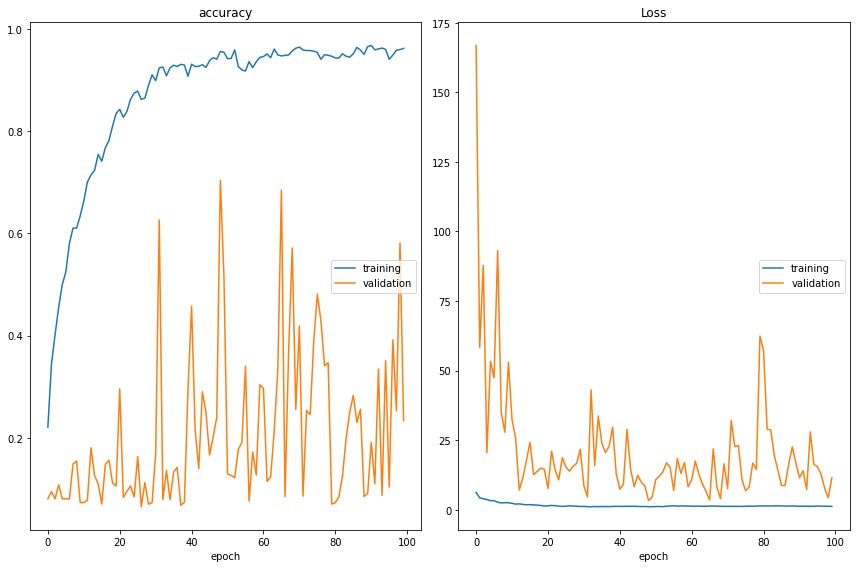
\includegraphics[width=\textwidth]{../figs/adam_acc_loss_100.png}
			\caption{Accuracy and Loss of the model using Adam Optimization Algorithm without Augmentation.}
			\label{img:adam_100}
		\end{figure}
		
		\begin{figure}
			\centering
			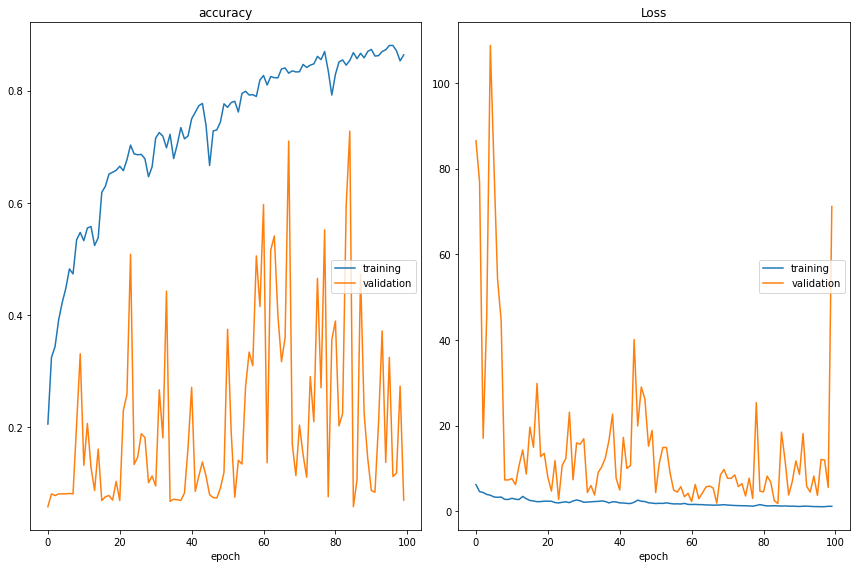
\includegraphics[width=\textwidth]{../figs/adam_aug_acc_loss_100.png}
			\caption{Accuracy and Loss of the model using Adam Optimization Algorithm using Augmentation.}
			\label{img:adam_aug_100}
		\end{figure}
		
		\section{Conclusion}
		%		data imbalance, no overfit 
		
		To conclude, all three optimizers almost take the time to train around 15 seconds for each iteration when running on a Google Colaboratory GPU. By applying data augmentation, the training time will increase to 17 seconds per epoch. Considering the values for the accuracies, this increase in the processing time does not make sense. Therefore, I believe that other methods have to be applied such as cross-validation. Moreover, better separation of the training and testing datasets has to be applied before going for data augmentation. 
		Comparing the results of two Adam Optimizers with the different number of epochs, the increase in the accuracy from 50 to 100 iterations, first of all, indicates that even with a high fluctuation of accuracy shown in all the figures, the training is not facing over-fitting. Secondly, it shows that we can still increase the number of iterations to achieve higher accuracy. 
		Finally, it seems that the performance of the Adam optimizer is the best among these three. After that, SGD is having a higher efficacy than RMS-Prop.
		The code is \href{https://colab.research.google.com/drive/1vs7KYJjMphoGcK-9g3tKnQ49ZFdIiYI5#scrollTo=p_ujrM0L4yR9}{linked here}.
		
		
		
	\end{proof}
	%
	%\bibliography{bibfile} 
	%\bibliographystyle{ieeetr}
	
\end{document}